%*****************************************
\chapter{Evaluation}\label{ch:evaluation}
%*****************************************

Test data was generated on a laptop running Linux Mint 10.0 using a 1.46 Ghz Intel Pentium dual core CPU with 1 GiB of RAM. A 10 Mbpbs broaband connection was used to connect to the internet, with measured download/upload rates of around 8 Mbps and 2 Mbps respectively.

For comparison, Firefox 4.0's minumum requirements include a single core 1.4 Ghz CPU with 512Mb of RAM \cite{firefox-req}. The average broadband speed in the UK is around 10 Mbps \cite{bband-stats}. 

\section{Image coding method}

We investigate how the concrete {\tt IConduitImage} implementation affects bit error rates and theoretical image capacity. The capacity puts a maximum limit on the number of possible recipients an image can be shared with, and also limits the size of the image. In addition, error rates determine which error correction schemes are most suitable and what the final output error rate will be after application of a given scheme.

We test the hypothesis that the HWT, 3-bit scaling and 4-bit scaling methods provide both greater capacity and lower error rates than the naive methods described in Section XXX after undergoing Facebook's image upload process.

\subsection{Method}

In this instance, local simulation with {\tt libjpeg} was used since uploading to Facebook on this scale would be considerably time consuming, and possibly warrant account deletion due to violation of Facebook's terms. We compress over the quality factor interval 80-90, since though it is most likely that Facebook uses IGJ quality factor 85, this is only an estimate. This also means our results are somewhat robust to minor changes in Facebook's compression process.

We model the compression/decompression process as a binary symmetric channel and calculate the channel capacity for arbitrarily small error probability, using an empirically measured bit error rate as an estimate for the bit error probability.

We write random input bytes to a $720 \times 720$ conduit image instance until full. The image is then saved as JPEG at a given quality factor, reloaded and the data extracted. We log the Hamming distance between the input and output data. This process is repeated until the cumulative amount of data processed exceeds 1 GiB. The test was performed for each of the three conduit image classes and also for quality factors 80-90.

\begin{table}[tbph]
  \begin{center}
        \begin{tabular}{l l l l l}
        \textbf{Method} &\textbf{Bits per} &\textbf{Test set size} & \textbf{Test set size} &\textbf{Possible unique} \\ 
            &\textbf{block} &\textbf{(images)} &\textbf{(blocks)} &\textbf{blocks} \\ [0.1ex] \hline \\ [-1.5ex]
        Scaled3	&192	&5,523	&44,736,300	& $6.28 \times 10^{57}$ \\
        Scaled4	&256	&4,142	&33,550,200	& $1.16 \times 10^{77}$ \\
        Haar	&24	&44,186	&357,906,600	& $1.68 \times 10^{7}$ \\
        \end{tabular}
        \caption{Tabulated details of the testing process. \textasciitilde 1 GiB of data was used for every test run.}
        \label{tab:img-test}
    \end{center}
\end{table}

Table \ref{tab:img-test} summerises the number of useful bits each method can store in a single 64 x 8 bit greyscale JPEG luminance block along with the effective sample size (number of images/blocks processed during the test) and population size (total number of possible unique blocks) we are sampling from. Due to the size of the samples the standard error is negligable, even before applying finite population correction where appropriate \footnote{In particular, for the Haar wavelet transform method the number of JPEG blocks encoded exceeds the number of unique datapoints that can be encoded in a single block.}. 

\subsection{Theoretical capacity calculation}

The per-image theoretical capacity is a function of the number of bits available per image $A$, given the implementation, and the bit error propability $p_e$:

\begin{equation}
    C = A \cdot (1 + H(p_e))
\end{equation}

where $H(x)$ is the binary entropy function. This provides the capacity in units of information per symbol - in our case KiB per image.

\subsection{Results}

Both n-bit scaling methods showed marked improvements in error rates and capacity (see Figure \ref{graph:ber} and Figure \ref{graph:capacity}) in comparison to naive approaches.

The HWT method, however, had the lowest capacity of all methods tested. We attribute this mainly to the fact that two passes of the HWT were required to succesfully reduce error rates, and that, due to the nature of the method, each pass reduces capacity by factor 4. The final error rates obtained were lower than all other methods, aside from 3-bit scaling which does at least support the claim made in XXX that such an encoding scheme is reasonably immune to JPEG compression.


\begin{figure}[tbph]
  \begin{center}
\begin{tikzpicture}
    \begin{axis}[grid=major,xlabel=JPEG Quality Factor,ylabel=BER (\%), xmin=80, xmax=90,
    height=8cm,width=10cm,legend style={legend pos=outer north east}]
    \addplot
        table[x=QF,y=Sc3] {gfx/error_rate.data};
    \addplot
        table[x=QF,y=Sc4] {gfx/error_rate.data};
    \addplot[mark=diamond*, color=green]
        table[x=QF,y=Haar] {gfx/error_rate.data};
        
    \addplot[mark=triangle*, color=purple]
        table[x=QF,y=rgb] {gfx/error_rate0.data};
    \addplot[mark=diamond*, color=orange]
        table[x=QF,y=dct] {gfx/error_rate0.data};
    
    \legend{Scaled3,Scaled4,Haar,Pixels,DCT}
    \end{axis}
\end{tikzpicture}
    \caption{Bit error rate for varying quality factors.}
    \label{graph:ber}
  \end{center}
\end{figure}

\begin{figure}[tbph]
  \begin{center}
\begin{tikzpicture}

    \begin{axis}[grid=major,xlabel=JPEG Quality Factor,ylabel=Capacity (KiB/image), xmin=80, xmax=90,
    height=8cm,width=10cm,legend style={legend pos=outer north east }]
    \addplot
        table[x=QF,y=Sc3] {gfx/encoding_time.data};
    \addplot
        table[x=QF,y=Sc4] {gfx/encoding_time.data};
    \addplot[mark=|, color=green]
        table[x=QF,y=Haar] {gfx/encoding_time.data};
        
    \addplot[mark=triangle*, color=purple]
        table[x=QF,y=rgb2] {gfx/error_rate0.data};
    \addplot[mark=diamond*, color=orange]
        table[x=QF,y=dct2] {gfx/error_rate0.data};
        
    \legend{Scaled3,Scaled4,Haar,Pixels,DCT}
    \end{axis}
\end{tikzpicture}
    \caption{Per-image channel capacity (measured in KiB/image) for varying quality factors.}
    \label{graph:capacity}
  \end{center}
\end{figure}

\subsection{Implications}

We can compare the capacity limit obtained in the previous section to the actual capacity achieved when an error correction scheme is applied, using quality factor 85 (see Table \ref{tab:fec}).

We can also use the estimation of bit error probability to calculate the probability of decoder output error. Given the bit error probability $p$ we can obtain the symbol error probability $p_s$:

\begin{equation}
    p_s = 1 - (1-p)^m
\end{equation}

where $m$ is the number of bits per symbol. In general, for a Reed Solomon code with symbol error probability $p_s$ the decoded symbol error probability $p_s'$ is given by:

\begin{equation}
    p_s' = \frac{1}{2^m -1} \sum^{2^m - 1}_{i = t+1} i {{2^m - 1}\choose{i}} {p_s}^i (1-{p_s})^{2^m - 1 - i}
\end{equation}

where $t$ is the maximum number symbol errors we can correct \cite{rsfec-decode}. The resulting decoder output error rates, along with achievable capacity, are shown in Table \ref{tab:fec}.

\begin{table}[tbph]
  \begin{center}
        \begin{tabular}{l l l l l l}
            
            \textbf{Method} & \textbf{FEC} & \textbf{$p$} & \textbf{$p_s$} & \textbf{$p_s'$} & \textbf{Capacity} \\  & &  &  &  & \textbf{(KiB)} \\[0.1ex] \hline \\ [-1.5ex]

            Haar & (15,9) & $4.20 \times 10^{-3}$ & $1.67 \times 10^{-2}$ & $2.47 \times 10^{-5}$ & 14.2 \\
            Haar &  (255,223) & $4.20 \times 10^{-3}$ & $3.31 \times 10^{-2}$ & $3.73 \times 10^{-4}$ & 20.8 \\
            Scaled3 & (15,9) & $8.30 \times 10^{-4}$ & $3.32 \times 10^{-3}$ & $4.28 \times 10^{-8}
$ & 113.9 \\
            \rowcolor{green!20!white} Scaled3 & (255,223) & $8.30 \times 10^{-4}$ & $6.62 \times 10^{-3}$ & $1.81 \times 10^{-13}
$ & 166.0 \\
            Scaled4 & (15,9) & $4.49 \times 10^{-2}$ & $1.68 \times 10^{-1}$ & $7.14 \times 10^{-1}$ & 151.9 \\
            Scaled4 & (255,223) & $4.49 \times 10^{-2}$ & $3.08 \times 10^{-1}$ & $3.08
 \times 10^{-1}$ & 221.4 \\
            
        \end{tabular}
        \caption{Bit error probability, symbol error probability and output symbol error probability for each possible combination.}
        \label{tab:fec}
    \end{center}
\end{table}

The 4-bit-per-pixel 'Scaled4' class produces a bit error rate too high to be corrected with the Reed Solomon codes used here, and indicates that a different FEC scheme would be appropriate.

Using the 3-bit-per-pixel 'Scaled3' class along with Reed Solomon (255,223) codes (highlighted in green) we would expect less than one bit error in a terrabyte of encoded data. For comparison, this approaches hard disk drive read error rates \footnote{Stated by at least one hard drive vendor to be 1 uncorrectable read error in $10^{14}$ bits, or 10 terabytes \cite{hdd-errors}.}. For these reasons the remainder of the evaluation will focus on this implementation.














\FloatBarrier
\section{Recipient group size}

We investigate how recipient group size affects encoding and decoding performance. Large or highly variable decoding times would have an adverse effect on usebility, in particular since decoding is triggered automatically whilst browsing.

Currently, all images are $720 \times 720$ pixels in size, and excess space is padded with random bytes for aesthetic effect. Recipient group size should therefore have little effect on the image coding times or output file size.

A preliminary analysis of retrieval and submission (shown in Figure XXX) indicates that overall encode and decode times are several orders of magnitude greater than the measurements of encryption times tabulated in Section XXX. We would therefore expect that overall codec performance will be roughly constant regardless of recipient group sizes.

\begin{figure}[tbph]
    \begin{center}
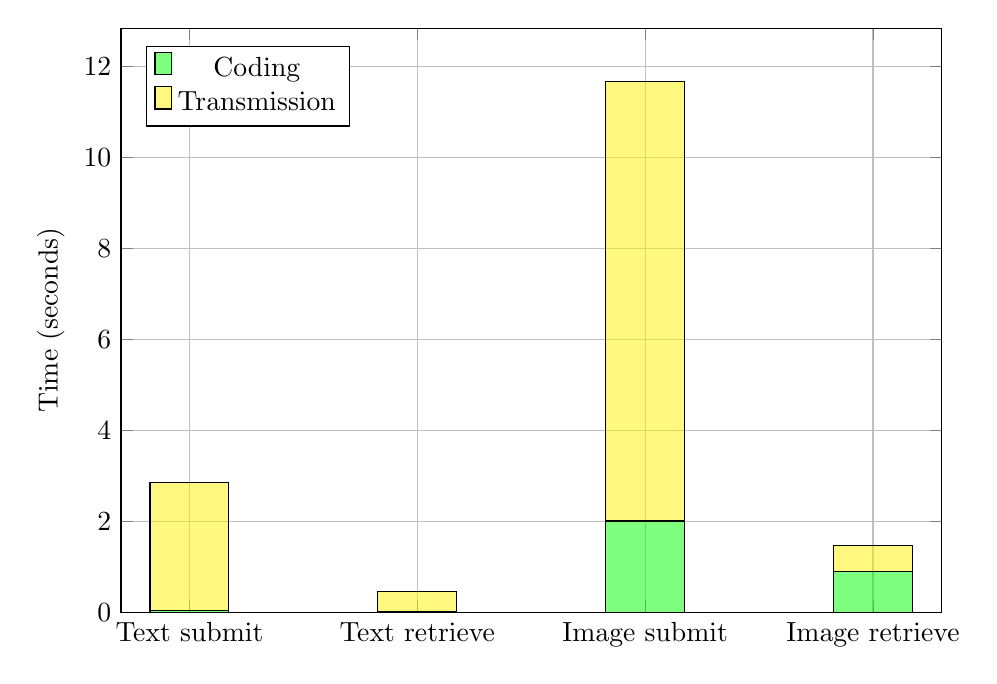
\begin{tikzpicture}
\begin{axis}[grid=major,ybar stacked, 
    symbolic x coords={Text submit,Text retrieve, Image submit, Image retrieve},
    xtick=data,ylabel=Time (seconds), width=12cm, height=9cm,
    legend style={legend pos=north west, area legend},
    bar width=1cm, ymin=0]

    \addplot[fill=green, fill opacity=0.5] coordinates
    {(Text submit,0.0444) (Text retrieve,0.0172) (Image submit,2.0074) (Image retrieve,0.9044)};
    
    \addplot[fill=yellow, fill opacity=0.5] coordinates
    {(Text submit,2.8013) (Text retrieve,0.4446) (Image submit,9.6655) (Image retrieve,0.5662)};
    
    \legend{Coding,Transmission}

\end{axis}
\end{tikzpicture}
    \caption{Average timing results for a 10,000 chracter note and an (approximately) 50 KiB image.}
    \label{graph:txt-sync}
  \end{center}
\end{figure}

We test the hypothesis that recipient group size has a negligeable effect on image codec performance.


\subsection{Method}

A 50 KiB random test vector was encrypted with 248-bit AES and 2048-bit RSA and encoded into an image\footnote{Using Scaled3 and (255,223) Reed Solomon codes.} and written out to disk in a lossless image format. For each test the number of recipients was increased up to 400. Recipients were duplicates and chosen randomly out of a pool of 15. The
image was then compressed using {\tt libjpeg}, then loaded and the data decoded. Encode and decode times were recorded and included writing to and from disk but not JPEG compression. 

\subsection{Results}




\begin{figure}[tbph]
    \begin{center}
    
\begin{tikzpicture}
\begin{axis}[grid=major,
    xlabel=Recipient group size, ylabel=Encoding Time (seconds), height=9cm,width=11cm,
    ymin=0, xmin=0, xmax=400, legend style={legend pos=north west, empty legend}]
    
    \addplot[only marks, mark=x] table[x=r,y=t]
        {gfx/submit.data};

    \addplot[no marks] table[x=r,y={create col/linear regression={y=t}}]
        {gfx/submit.data};
        
    \addlegendentry{Slope = $\pgfmathprintnumber{\pgfplotstableregressiona}$};
    \addlegendentry{R = $\pgfmathprintnumber{0.726}$}

\end{axis}
\end{tikzpicture}

\begin{tikzpicture}
\begin{axis}[grid=major,
    xlabel=Recipient group size, ylabel=Decoding Time (seconds), height=9cm,width=11cm,
    ymin=0, xmin=0, xmax=400, legend style={legend pos=north west, empty legend}]
    
    \addplot[only marks,mark=x] table[x=r,y=t]
        {gfx/retrieve.data};
    
    \addplot[no marks] table[x=r,y={create col/linear regression={y=t}}]
        {gfx/retrieve.data};

    \addlegendentry{Slope = $\pgfmathprintnumber{\pgfplotstableregressiona}$};
    \addlegendentry{R = $\pgfmathprintnumber{0.846}$}

\end{axis}
\end{tikzpicture}

    \caption{Encoding (top) and decoding (bottom) times as recipient numbers increase.}
    \label{graph:subrep}
  \end{center}
\end{figure}

\section{Implications}





\section{Plaintext caching}

We investigate the effect of clearing the extension cache on page loading times. Due to the nature of the parsing process (see Section XXX) a cache of plaintext content accumulates on the user's machine. Currently this cache is wiped on initialisation and destruction. It would be possible to decrease the period between cache expiration, perhaps for better security\footnote{Though attacks involving the cache are not included in our initial threat model, mainly because they involve access to the user's machine.} or for decreased local storage utilisation. Increasing the cache period would likely lead to smaller amortised page loading times, which would benefit usebility. In either case it would be useful to know the maximum beneficial effect clearing the cache can have on page loading times.

We test the hypothesis that clearing the plaintext cache increases page load times, and estimate by what factor times are increased for a page full of encrypted items.


\subsection{Method}

Sample newsfeeds were generated with 15 encrypted status update entries, as this is the number of newsfeed entries Facebook first loads \footnote{More are loaded dynamically when the user scrolls to the bottom of the page.}. Status update messages were random ASCII text 420 characters in length, the maximum permitted. The pages were loaded repeatedly 400 times, ensuring that both the browser cache and extension cache were cleaned after each load.

The entire process was then repeated for a newsfeed containing 15 image objects, once again random images of size 50 KiB, instead of status messages. A second set of test were performed without cleaning the extension cache (which was preloaded with the page's content).

The start time of each test was logged, along with the subsequent load times of the encrypted objects. 

    \begin{figure}[tbph]
        \begin{center}
                
\includegraphics[width=10cm]{screens/parrots1.png}
                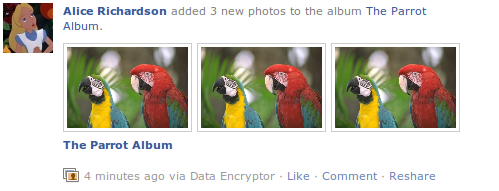
\includegraphics[width=10cm]{screens/parrots2.png}
            \caption{Newsfeed excerpt containing encrypted image thumbnails, before (top) and after (bottom) parsing.}
            \label{scn:parrots}
        \end{center}
    \end{figure}


\subsection{Results}

The effect of plaintext caching on the overall page loading times can be seen in figure \ref{graph:hist}. On average, caching provided a greater than factor 2 speed increase for text and a factor 5 increase for images.

\begin{figure}[tbph]
    \begin{center}
\begin{tikzpicture}
\begin{axis}[xlabel=Time (seconds), ylabel=Frequency,
grid=major,const plot, ymin=0, enlargelimits=false,
width=12cm, height=5cm, legend style={area legend}]

    \addplot[fill=blue, fill opacity=0.5] table[x=t,y=Text] {gfx/async_text_hist.data};
    
    \addplot[fill=red, fill opacity=0.5] table[x=t,y=Text_c] {gfx/async_text_hist.data};
    
    \addplot+[sharp plot,blue, mark=no marker] coordinates
        {(6.403,0) (6.403,56)};
        
    \addplot+[sharp plot,red, mark=no marker] coordinates
        {(3.463,0) (3.463,56)};
    
    \legend{Cache off,Cache on}
\end{axis}
\end{tikzpicture}

\begin{tikzpicture}
\begin{axis}[xlabel=Time (seconds), ylabel=Frequency,
grid=major,const plot, ymin=0, enlargelimits=false,
width=12cm, height=5cm, legend style={area legend}]
    
    \addplot[fill=blue, fill opacity=0.5] table[x=t,y=Images] {gfx/async_image_hist.data};
    
    \addplot[fill=red, fill opacity=0.5] table[x=t,y=Images_c] {gfx/async_image_hist.data};
    
    \addplot+[sharp plot,blue, mark=no marker] coordinates
        {(19.169,0) (19.169,130)};

    \addplot+[sharp plot,red, mark=no marker] coordinates
        {(4.067,0) (4.067,130)};
    
    \legend{Cache off,Cache on}
    
\end{axis}
\end{tikzpicture}
    \caption{Histogram of 400 page loading times for newsfeeds containing 15 encrypted messages (top) and 15 encrypted images (bottom).}
    \label{graph:hist}
  \end{center}
\end{figure}

After the first item has loaded we can also look at the waiting time between loads. The most dramatic increase is for image, as seen on Figure XXX. Full breakdowns of timings with and without the cache are inlcluded in Appendix XXX.

\begin{figure}[tbph]
\begin{center}
    
\begin{tikzpicture}
\begin{axis}[grid=major,ycomb,
ylabel=Time (ms), 
width=12cm, height=5cm,
bar width=0.3cm, ymin=0, xmin=2, xmax=15, enlarge x limits=0.04]
    \addplot[blue] table[x=Item,y=Image] {gfx/async.data};
\end{axis}
\end{tikzpicture}

\begin{tikzpicture}
\begin{axis}[grid=major,ycomb,
ylabel=Time (ms),xlabel=Image,
width=12cm, height=5cm,
bar width=0.3cm, ymin=0, xmin=2, xmax=15, enlarge x limits=0.04]
    \addplot[red,] table[x=Item,y=Image_c] {gfx/async.data};
\end{axis}
\end{tikzpicture}

\caption{Average time interval between successive image loads, with caching turned off and on (top and bottom respectively).}
\label{graph:img-rest}
\end{center}
\end{figure}


\subsection{Implications}

Based on the results, most users would likely benefit from cleansing the cache as little as possible, unless a user was particularly security conscious and used the extension mainly for text communications rather than image sharing. A full study of how the size of the cache increases in size over time would also be appropriate; this was unfortunately not possible in the limited evaluation timeframe.


\section{Usebility inspection}

We investigate the outcome of the ongoing usebility inspection that was used as part of the development process, in particular since usebility was a goal from the outset.

Comments and Images are two of the most frequently shared forms of content (see Section XXX). The submission processes for Comments and Images are also two of the most convoluted processes required of a user. Appendix XXX details usebility inpsections of many other processes in detail.

We test the hypothesis that a typical Facebook user can sucessfully encrypt and share an encrypted Image, and that a simiair user can succesfully submit an encrypted Comment on that image.


\subsection{Method}


\subsection{Results}

A full user study was considered too time consuming to perform; instead we use a cognitive walkthrough (as described by Wharton et al \cite{cogwalk}) to evaluate the success of the user interface. This section consists of a selection of some of the final success stories and a defense of their validity. They refer to claims demonstrated by other walkthroughs which can be found Appendix XXX.

We only consider one class of user - a typical Facebook user who is therefore familiar with the Facebook user interface. It is therefore assumed that actions such as "navigate to a given friend's profile" can be performed without additional aid. It is also assumed that the user will follow their usual actions when trying to perform an encrypted operation - when trying to upload an encrypted image they will, for example, simply follow the normal procedure for uploading an image rather than searching for some hidden option. Finally, we make the assumption that the extension has been installed and enabled and that the toolbar has not been hidden.


\subsection{Uploading an encrypted image}
A user wishing to send an encrypted image to 405 friends who also have the extension, does so.

\begin{desc}

    \item[Action Sequence] \hfill
    \begin{enumerate}
        \item Add any public keys required.
        \item Navigate to the image upload page for the required album (see Figure \ref{scn:pic-up}).
        \item Select the image to encrypted.
        \item Check the {\tt [Encrypt]} check box.
        \item Click the {\tt [Submit]} button.
        \item Use the friend selector to select recipients and submit.
    \end{enumerate}
    
    \item[Defense of Credibility] \hfill
        \begin{itemize}
            
            \item The user knows he must add punlic keys of recipients beforehand and how to do so. If the user has no public keys section XXX demonstrates that he will be able to add one of his intended recipients. Since the process is reasonably simple - simply navigate to their page and click a clearly marked button, we assume that any user who has performed it once can do so again if they wish, without further instruction. The link between adding public keys and being able to choose those friends as recipients should be fairly obvious; when the first key is added and encryption attempted again that same friend will appear as the only possible recipient.
            
            \item Facebook user will be familiar with the process of uploading an image. We assume a user trying to upload an encrypted image will be likely to try the method they are already familiar with.
            
            \item User knows things are OK since he sees the encryption check box option on arriving at the upload page. Check box leaves little room for confusion over whether an upload will or won't be encrypted.
            
            \item User knows to select an image to upload since the process is identical to uploading plaintext images.
            
            \item User knows to select {\tt [Encrypt]} check box since uploading an encrypted image is the original task.
            
            \item User knows things are OK since the recipient selector pops up.
            
            \item User knows how to use the recipient selector (see section XXX).
            
            \item User knows things are OK as Facebook handles the upload process from here as per normal, notifying user when the upload is complete.
            
        \end{itemize}
    
\end{desc}


    \begin{figure}[tbph]
        \begin{center}
        
                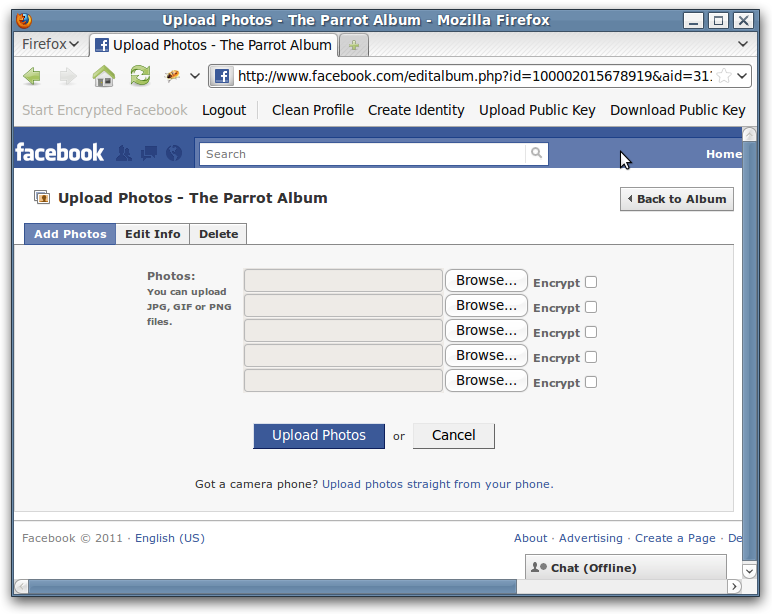
\includegraphics[width=12cm]{screens/pic-upload.png}

            \caption{Input fields and controls for submitting encrypted images.}
            \label{scn:pic-up}
        \end{center}
    \end{figure}

\subsection{Posting a comment}
A user has navigated to his newsfeed. He wishes to write an encrypted reply to a plaintext comment on a newsfeed post of an encrypted photo. It is assumed he already possesses the public keys required and can decrypt the photo in question.

\begin{desc}

    \item[Action Sequence] \hfill
    \begin{enumerate}
        \item Select the comment box below the plaintext reply.
        \item Type comment in plaintext.
        \item Click the {\tt [Encrypt \& Submit]} button.
        \item Use the friend selector to select recipients and submit.
        \item Refresh the page to review comment.
    \end{enumerate}
    
    \item[Defense of Credibility] \hfill
        \begin{itemize}
            
            \item User knows to select the comment box. This is required for submitting a plaintext comment, we assume the user will try the method they are used to.
            
            \item User knows things are OK as the {\tt [Encrypt \& Submit]} appears once the textbox has focus.
            
            \item User knows to type in the comment - this is identical to submitting a plaintext comment.
            
            \item User knows to click {\tt [Encrypt \& Submit]}. The user is familiar with clicking a similiar submit button during plaintext entry. The button is positioned beside the {\tt [Submit]} for plaintext entry, is styled like the {\tt [Submit]} button and is clearly labelled. Submitting an encrypted comment is part of the original task.
            
            \item User knows how to use the recipient selector (see section XXX).
            
            \item User knows things are OK as Facebook handles the submission process from here as per normal. A loading icon appears breifly, then the comment itself appears.
            
            \item User knows that their submission was encrypted as this fact is stated as part of the comment encoding.
            
            \item User knows they must refresh the page to view their own comment. Even if this is their first encrypted submission, Facebook users will be familiar with the process of refreshing a page when something is not working or to view an update. If the user does not make the connection right away, when returning to the page and seeing the item decrypted automatically they should realise that encrypted text submissions are decrypted as a page first loads.
        
        \end{itemize}
\end{desc}


    \begin{figure}[tbph]
        \begin{center}
        
                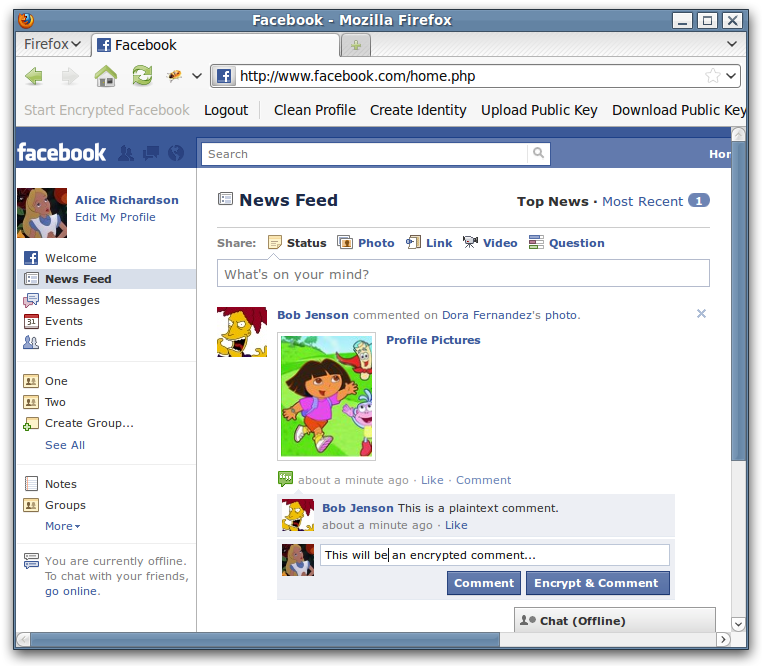
\includegraphics[width=12cm]{screens/comment.png}

            \caption{Input fields and controls for posting a comment to a newsfeed entry.}
            \label{scn:comment}
        \end{center}
    \end{figure}























\section{Conduit image performance}

The per-image channel capacity is a the function of the amount of information the implementation can store in a single image (equivalently - the symbol size) and the bit error probability. We model the compression/decompression process as a binary symmetric channel and calculate the channel capacity for arbitrarily small error probability, using the empirical bit error rate as an estimate for the bit error probability.

When used in conjunction with a forward error correction scheme we can also consider the actual per-image useful data rate and final decoder output error probability.


\subsection{Method}

The relevant library components are loaded into a test C++ application. A standalone conduit image instance is created and a random byte vector generated and encoded. The result is saved to disk as a JPEG at a given quality factor, reloaded and the data decoded. We log the Hamming distance between the input and output data. This process is repeated until the cumulative amount of data processed exceeds 1 GiB. The test was repeated for each of the three conduit image classes and also for quality factors 80-90.



Table \ref{tab:img-test} summerises the number of useful bits each method can store in a single 64 x 8 bit greyscale JPEG luminance block along with the effective sample size (number of images/blocks processed during the test) and population size (total number of possible unique blocks) we are sampling from. Due to the size of the samples the standard error is negligable, even before applying finite population correction where appropriate \footnote{In particular, for the Haar wavelet transform method the number of JPEG blocks encoded exceeds the number of unique datapoints that can be encoded in a single block.}.




\subsection{Theoretical capacity}
\label{ssec:capacity}


Figure \ref{graph:ber} charts bit error rates for each implementation. As expected, rates generally decrease as the quality factor increases. Both n-bits scaling methods show a marked improvement over the naive approaches in Section \ref{ssec:naive}.



We model each conduit image as a binary symmetric channel: we know the encoding/decoding process does not result in bit erasures; we make the assumption that the probability of error $p_e$ is independant and equal for each bit. Given the large sample sizes we can assume that the measured bit error rate is a reasonable estimate of the actual bit error probability.

The formula used to calculate the capacity is obtained by taking the typical capacity calculation for a binary symmetric channel and multiplying by the number of bits available per image $A$, to obtain:

\begin{equation}
    C = A \cdot (1 + H(p_e))
\end{equation}

Where $H(x)$ is the binary entropy function. This provides the capacity in units of information per symbol - in this case bits per image. Figure \ref{graph:capacity} compares the calculated capacity for each of the three conduit images implementations. At quality factor 85, which most closely matches the profile of the Facebook JPEG compression proccess, we see both scaling methods performing approximately the same with capacities of over 180 KiB per image.


\subsection{Reed Solomon error correction}

Given the bit error probability $p$ we can obtain the symbol error probability $p_s$:

\begin{equation}
    p_s = 1 - (1-p)^m
\end{equation}

where $m$ is the number of bits per symbol. In general, for a Reed Solomon code with symbol error probability $p_s$ the decoded symbol error probability $p_s'$ is given by:

\begin{equation}
    p_s' = \frac{1}{2^m -1} \sum^{2^m - 1}_{i = t+1} i {{2^m - 1}\choose{i}} {p_s}^i (1-{p_s})^{2^m - 1 - i}
\end{equation}

where $t$ is the maximum number symbol errors we can correct \cite{rsfec-decode}. Both the error correction classes in the Encrypted Facebook library are based on Reed Solomon codes. The (15,9) code can correct up to $t=3$ symbol errors and has a 4-bit symbol size. The (255,223) code can correct up to $t=16$ symbol errors and has a 8-bit symbol size.

Figure \ref{tab:fec} tabulates error probabilities for each FEC scheme used; again we use the
measured bit error rate as an estimate of the bit error probability. The decoded symbol error probability $p_s'$ we may consider as an upper bound for the decoded bit error probability. 



\subsection{Conclusion}
\label{ssec:image-conc}

The Haar wavelet class has too low a capacity (at any quality factor) to be used in practise, though the low bit error rates logged support the claim (see XXX) that such an encoding is reasonably immune to JPEG compression. In addition, there is anecdotal evidence that suggests that $p_s'$ in Figure \ref{tab:fec} is not a particularly tight bound on the actual output bit error probability - during the testing in section XXX several megabytes of data were encoded, uploaded and retrieved successfuly. 

The 4-bit-per-pixel 'Scaled4' class produced a bit error rate too high to be corrected with the Reed Solomon codes used here. Implementing a forward error scheme with a lower code rate would make this feasible - in particular if the JPEG quality factor were higher than 85 this method could potentially offer the highest capacity of the three classes tested.

The 3-bit-per-pixel 'Scaled3' class along with Reed Solomon (255,223) codes (highlighted in green) demonstrates a feasible combination (see XXX). Under this scheme we would expect less than one bit error in a terrabyte of encoded data. For comparison, this approaches hard disk drive read error rates \footnote{Stated by at least one hard drive vendor to be 1 uncorrectable read error in $10^{14}$ bits, or 10 terabytes \cite{hdd-errors}.}. For these reasons the remainder of the evaluation will focus on this implementation.



\section{Submission and retrieval times}

We consider the encode/decode and upload/download times for a single object, encoded using the 'Scaled3' class. Effects of asynchronous retrieval of multiple objects and caching of plaintext information locally are covered in section XXX.  


\subsection{Method}

Automated tests were ran programmatically from the extension, with each submission and retrieval round being allowed to complete entirely before beginning the next. All encryption was performed with a simulated group size of 405 as detailed in section XXX. Test images were duplicate copies of a (approximately) 50 KiB JPEG image (see section XXX). Test messages were randomly generated strings of mixed-case letter and numeral characters, 10,000 characters in length - the limit for private messages.

For textual content, 1000 messages were generated. The note submission function was then called with each message using a 60 second delay in between each run - leaving enough time for one submission and retrieval round to complete before beginning another. The tags required to retrieve these notes are saved and the time spent in each submission phase profiled. When the HTTP request for sumbmission completes, retrieval is triggered and the download and decoding time logged. The same test was repeated using a set of 1000 images.

All retrieved objects were compared with the originals to ensure error free transfer had occured. A modified version of the Chromebug Firefox extension was used to record all results.


\subsection{Results}

For text messages times were dominated by the HTTP transfer; encoding and decoding times were negligable. For images the encoding and decoding times were more significant, in particular when retrieveing where more time was spent decoding the image than downloading.

\begin{figure}[tbph]
    \begin{center}
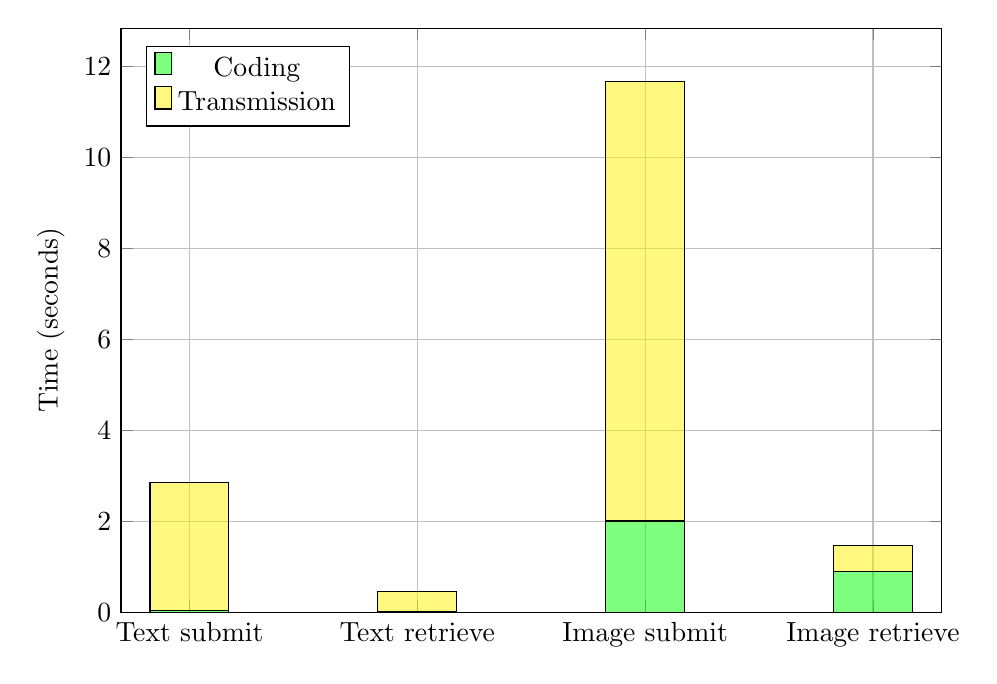
\begin{tikzpicture}
\begin{axis}[grid=major,ybar stacked, 
    symbolic x coords={Text submit,Text retrieve, Image submit, Image retrieve},
    xtick=data,ylabel=Time (seconds), width=12cm, height=9cm,
    legend style={legend pos=north west, area legend},
    bar width=1cm, ymin=0]

    \addplot[fill=green, fill opacity=0.5] coordinates
    {(Text submit,0.0444) (Text retrieve,0.0172) (Image submit,2.0074) (Image retrieve,0.9044)};
    
    \addplot[fill=yellow, fill opacity=0.5] coordinates
    {(Text submit,2.8013) (Text retrieve,0.4446) (Image submit,9.6655) (Image retrieve,0.5662)};
    
    \legend{Coding,Transmission}

\end{axis}
\end{tikzpicture}
    \caption{Average timing results for a 10,000 chracter note and an (approximately) 50 KiB image.}
    \label{graph:txt-sync}
  \end{center}
\end{figure}













\section{Effect of cache on loading times}

We evaluate the effect of caching plaintext items that have already been retreived when loading an entire page. Here we also condiser DOM tree navigation/insertion operations and asynchronous object retrieval. Pages containing multiple items of encrypted content were loaded, triggering asynchronous retrieval and deocoding.


\subsection{Method}

Sample newsfeeds were generated with 15 encrypted status update entries, as this is the number of newsfeed entries Facebook first loads \footnote{More are loaded dynamically when the user scrolls to the bottom of the page.}. Status update messages were random ASCII text 420 characters in length, the maximum permitted. The pages were loaded repeatedly 400 times, ensuring that both the browser cache and extension cache were cleaned after each load.

The entire process was then repeated for a newsfeed containing 15 image objects, once again random images of size 50 KiB, instead of status messages. In addition, a second set of test were performed without cleaning the extension cache (which was preloaded with the page's content).

The start time of each test was logged, along with the 15 subsequent load times of the encyrpted objects. 

    \begin{figure}[tbph]
        \begin{center}
                
\includegraphics[width=10cm]{screens/parrots1.png}
                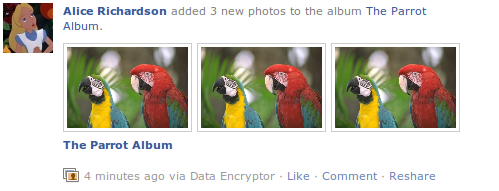
\includegraphics[width=10cm]{screens/parrots2.png}
            \caption{Newsfeed excerpt containing encrypted image thumbnails, before (top) and after (bottom) parsing.}
            \label{scn:parrots}
        \end{center}
    \end{figure}




